\section{Theoretical Framework}
\label{seq:theoretical-framework}

Nonlocal behaviours were first predicted and formulated in the context of entangled spin one-half particles \cite{epr}. 
With the establishment of Bell nonlocality as a standalone field, specific physical scenarios were replaced with more implementation-agnostic frameworks \cite{brunner}.
In this report, \emph{Bell scenarios}, first introduced by \citeauthor{bell_einstein_1964} in \citeyear{bell_einstein_1964} \cite{bell_einstein_1964}, are considered.

In a Bell scenario, two parties \emph{Alice} and \emph{Bob}, sharing
a quantum state $\ket{\psi}$ on which they can perform valid measurements $M$ and $N$, are considered. Each party has $m$ choices
of measurement and $\Delta$ possible outcomes. 

The \emph{outputs} are denoted
$(a,b)$ and the \emph{inputs} $(x,y)$, as
is depicted in \Autoref{fig:bell_scenario}. For the rest of the report, only Bell scenarios in which $\Delta = 2$ and $m \in \{2 ,3\}$ are considered.

\begin{figure}[h!]
  \centering
    \begin{tikzpicture}
    %%% Alice
    % big square
    \node (alice) [fill = gray!20, draw = gray!70,line width = 0.75mm, minimum size=2cm, draw, rounded corners = 0.15cm] at (-2.5,0.0) {};
    % triangle
    \node [isosceles triangle, isosceles triangle apex angle=90, line width=0.5mm, rotate=180, minimum size=0.25cm, draw, fill=teal!40] at (-2.15, 0.0) {};
    % measuring device
    \node (a_measure) [fill = teal!40, line width=0.5mm, minimum size=1cm, draw, rounded corners = 0.1cm] at (-2.70, 0.0) {$M_{a | x}$};
    % receive x
    \draw [-to, line width=0.5mm, rounded corners= 0.05cm] (-2.5, 1.5) node[above] {\large $x$} -- (-2.5, 0.85) -- (-2.70,0.85) -- (-2.70, 0.55);
    % output a
    \draw [-to, line width=0.5mm, rounded corners= 0.05cm] (-2.7, -0.55) -- (-2.7, -0.85) -- (-2.5, -0.85) -- (-2.5, -1.5) node[below] {\large $a$};

    %%% Bob
    % big square
    \node [fill = gray!20, draw = gray!70,line width = 0.75mm, minimum size=2cm, draw, rounded corners = 0.15cm] at (2.5, 0.0) {};
    % triangle
    \node [isosceles triangle, isosceles triangle apex angle=90, line width=0.5mm, minimum size=0.25cm, draw, fill=purple!40] at (2.15, 0.0) {};
    % measuring device
    \node [fill = purple!40, line width=0.5mm, minimum size=1cm, draw, rounded corners = 0.1cm] at (2.7, 0.0) {$N_{b | y}$};
    % receive y
    \draw [-to, line width=0.5mm, rounded corners= 0.05cm] (2.5, 1.5) node[above] {\large $y$} -- (2.5, 0.85) -- (2.70,0.85) -- (2.70, 0.55);
    % output b
    \draw [-to, line width=0.5mm, rounded corners= 0.05cm] (2.7, -0.55) -- (2.7, -0.85) -- (2.5, -0.85) -- (2.5, -1.5) node[below] {\large$b$};

    %%% Entanglement sharing
    % photon source
    \node (psi) [line width=0.5mm, rounded corners = 0.05cm, draw, label={south: \large$\ket{\psi}$}] {Source};
    % line to A
    \draw[decorate, decoration={snake}, line width = 0.5mm] (-1.65,0.0) -- (-0.75,0.0) node[above=4] {} -- (psi);
    % line to B
    \draw[decorate, decoration={snake}, line width = 0.5mm] (psi) -- (0.75,0.0) node[above=4] {} -- (1.65, 0.0);
    % prolong non-squiggly part of the line
    \draw[line width = 0.5mm] (-1.75, 0.0) -- (-1.65,0.0);
    \draw[line width = 0.5mm] (1.75, 0.0) -- (1.65,0.0);
    % draw circle at the end
    \draw[fill] (-1.75, 0.0) circle (.05cm);
    \draw[fill] (1.75, 0.0) circle (.05cm);
  \end{tikzpicture}

  \caption{Bell scenario; a quantum state $\ket{\psi}$ is shared between two parties Alice and Bob, who receive $x$ and $y$ and output $a$ and $b$ according to measurement operators $M_{a | x}$ and $N_{b | y}$, respectively.}
  \label{fig:bell_scenario}
\end{figure}

From one experiment to another, the outcomes $a$ and $b$ that are obtained may vary, 
even if Alice and Bob use the same measurement operators. As such, these outcomes can
be described via a \emph{probability distribution} \cite{brunner}. 

This elements of this probability distribution are referred to as \emph{joint probabilities}, and are denoted $p(a,b|x,y)$. The vector of all joint probabilities $\mathcal{P} = \{p(a,b|x,y)\}$ describes the operation of the Bell scenario and is referred to as the \emph{behaviour} (\sref{Definition}{def:behaviour}) or the \emph{correlations} of the scenario.

\begin{definition}[Behavior or correlations]
\label{def:behaviour}
A behavior or correlations is a
vector $\mathcal{P} = \{p(a,b|x,y)\}$ of all joint probabilities to obtain the output
pair $(a,b)$ given the input pair $(x,y)$. 
\end{definition} 

An interesting property of this definition, is that a behavior can be seen as a point $\mathcal{P}$ in the vector space $\mathbbm{R}^{\Delta^2 m^2}$. This property will be useful for the expression of behaviours with semi-definite programming in \Autoref{sec:nonloc-detection}.

To construct \emph{valid behaviours}, one must ensure that it verifies certain conditions: essentially, the behaviour must constitute a \emph{valid probability distribution} \cite{brunner}.

\begin{proposition}
A behaviour $\mathcal{P}$ must satisfy two conditions: it must be \emph{positive}, i.e.\ $\forall a, b, x, y$,
\begin{equation}\label{eq:norm_cons_1}
    p(a,b|x,y) \geq 0 \text{,}
\end{equation}
and it must be \emph{normalized}, i.e.\ $\forall x,y \in \{1,m\}$,
\begin{equation}\label{eq:norm_cons_2}
\sum_{a,b=1}^m p(a,b|x,y) = 1 \text{.}
\end{equation}
\end{proposition}

% \hpa{maybe put into convex polytopes}

Several types of behaviours exist: with this formalism, one can express both \emph{local}, \emph{quantum} and \emph{no-signalling} behaviours, respectively referred to by the probability spaces to which they belong: $\mathcal{L}$, $\mathcal{Q}$ and $\mathcal{NS}$ (this will be addressed in more detail in \Autoref{sec:char-corr}). 
In the rest of the report, the space $\mathcal{K} \in \{\mathcal{L}, \mathcal{Q}, \mathcal{NS}\}$ will be used to refer to the probability space of an arbitrary valid behaviour.

% In the following Considering the aforementioned vector space $\mathbb{R}^{\Delta^{2}m^{2}}$
% Three sets of specific type of correlations are included in the probability
% space: the set $\L$ of local correlations, the set $\Q$ of quantum
% correlations and the set of no-signalling correlations $\NS$.
% Throughout the report, we consider the set 
% $\mathcal{K} = \mathcal{L}, \mathcal{Q} \text{ or } \mathcal{NS}$. 

\subsection{Characterizing correlations}
\label{sec:char-corr}

When considering two distant observers $A$ and $B$ performing measurements on a shared physical system, correlations arise as an important property of the system \cite{bell-viol-self-test}.

In this subsection, both local, quantum and no-signaling correlations are described.

% One of the most notable characteristics of a quantum state is the way 

% \hpa{correlations belong to several distinct classes}

\subsubsection{Local correlations}

% \hpa{what do local correlations correspond to}
Local correlations correspond to behaviours that are allowed in classical physics: informally, they enforce the fact that the two observers $A$ and $B$ cannot communicate before outputting $a$ and $b$. \sref{Definition}{def:local-corr} formalizes this notion:

\begin{definition}[Local correlations]
\label{def:local-corr}
A behaviour $\mathcal{P}$ is said to be
local if its joint probabilities $p(a,b|x,y)$ can be written \begin{equation}
    p(a,b|x,y) = \int_\Lambda q(\lambda) p(a|x,\lambda)p(b|y,\lambda)
    \mathrm{d}\lambda
\end{equation} where $\lambda \in \Lambda$ are local hidden variables with a
probability density distribution $q(\lambda)$. Otherwise, the correlations are
non local. \\ \end{definition}

Local correlations can also be expressed in a simpler form, in terms of deterministic local hidden-variable models - in what is referred to as a local deterministic behaviour (\sref{Definition}{def:local-det-beh}). The equivalence of these two definitions follows from the fact any local randomness present in $p(a | x, \lambda)$ and $p(b | y, \lambda)$ can be incorporated in the shared random variable $\lambda$ \cite{brunner}.

\begin{definition}[Local deterministic behaviours]\label{def:local-det-beh} Let
$\lambda=(a_1,\ldots,a_m\,;\,b_1,\ldots,b_m)$ be the assignment of outputs
$a_x,b_y$ for each inputs possible. The corresponding deterministic behaviour is
\begin{equation}
    \mathbf{d_\lambda}(a,b|x,y) = \begin{cases} 1 & \text{if } a=a_x \text{ and
    } b=b_y \text{,}\\ 0 & otherwise \text{.} \end{cases}
\end{equation} There are $\Delta^{2m}$ possible deterministic behaviours.
\end{definition}

One can also give an inductive definition for local behaviours, which will be useful in the linear programming formulation of \Autoref{sec:nonloc-detection}:

\begin{proposition}[Local correlations] \label{convex_sum} A behaviour
$\mathcal{P}$ is local if and only if it can be written as a convex combination
of deterministic behaviours, i.e \begin{equation}
    \mathcal{P} = \sum_\lambda \mu_\lambda \mathbf{d}_\lambda \ , \ \mu_\lambda
    \geq 0 \ , \ \sum_\lambda \mu_\lambda = 1 \text{.}
\end{equation} \end{proposition}


\subsubsection{Quantum correlations}

Quantum correlations correspond to behaviours that are allowed in quantum mechanics: they can possess nonlocal characteristics \cite{bell-viol-self-test}.

% \hpa{what quantum correlations correspond to}

Let $\mathcal{H_A} \otimes \mathcal{H_B}$ be the joint Hilbert space of Alice
and Bob and $\rho_{AB}$ be the quantum states representing their shared physical
system. Let $\{M_{a|x}\}$ and $\{N_{b|y}\}$ be the sets of measurement operators
respectively on $\mathcal{H_A}$ and $\mathcal{H_B}$. These measurement operators satisfy
\begin{equation*}
\begin{aligned}
       \forall x,a,\ & M_{a|x} \succcurlyeq 0 & \text{ and } \ 
            & \forall x ,\ \sum_a  M_{a|x} = \mathbbm{1}_A \ , \\
       \forall y,b,\ & M_{b|y} \succcurlyeq 0 & \text{ and } \ 
            & \forall y ,\ \sum_b  M_{b|y} = \mathbbm{1}_B \ ,\\
\end{aligned}
\end{equation*}
therefore $\{M_{a|x}\}$ and $\{N_{b|y}\}$  characterize POVMs \cite{nielsen_quantum_2010}, and can thus be experimentally constructed.

The set of behaviours achievable in quantum mechanics $\mathcal{Q}$ corresponds to the set of behaviours who verify the following condition:

\begin{definition}[Quantum correlations] \label{eq:quant-correlation}

A behaviour $\mathcal{P}$ is quantum if
its elements can be written as 
\begin{equation}
    p(a,b|x,y) = \textrm{Tr}\left(  \rho_{AB}  M_{a|x} \otimes N_{b|y}\right)
\end{equation} 
\end{definition}

The previous definition works for pure states, but one can always consider a purification for arbitrary quantum states (\sref{Proposition}{prop:qu_corr}).

\begin{proposition} \label{prop:qu_corr} Without loss of generality, one can
take a purification $\Phi$ of $\rho_{AB}$ and consider $M_{a|x} ,N_{b|y}$ to be
orthogonal projectors. Hence, quantum behaviour elements can be written
\begin{equation}
        p(a,b|x,y) = \bra{\Phi}  M_{a|x} \otimes N_{b|y} \ket{\Phi} \text{.}
        \label{eq:qu_corr}
\end{equation} \end{proposition}



\subsubsection{No-signaling correlations}

No-signalling constraints state that the marginal probabilities $p(a|x)$ (respectively $p(b|y)$) are
independent of Bob's (respectively Alice's) measurement, i.e \emph{Bob and Alice cannot signal instantaneously
their outputs to each other by their choice of input} \cite{brunner}.
\begin{definition}[No-signalling correlations] A behaviour $\mathcal{P}$ is no-signalling if
its elements fulfill the following constraints
\begin{equation}
\begin{aligned}
    \forall \ a,x,y,y'\;  & \ \sum_{b=1}^\Delta p(a,b|x,y) & = &\ \sum_{b=1}^\Delta p(a,b|x,y')  \\
    \forall \ b,y,x,x'\;  & \ \sum_{a=1}^\Delta p(a,b|x,y) & = &\ \sum_{a=1}^\Delta p(a,b|x',y)
\end{aligned}
\end{equation} \end{definition}

\subsubsection{Correlation spaces and facet Bell inequalities}

The relationship between the three types of correlations can be visualized in \Autoref{fig:geometric-correlations}. While the no-signaling and local sets can be easily characterized, the set of quantum correlations is more difficult to describe \cite{bell-viol-self-test}, but the property in \sref{Proposition}{prop:corr} (introduced by \citeauthor{popescu_quantum_1994} in \cite{popescu_quantum_1994}) always holds.

\begin{figure}[t!]
    \centering
    \begin{tikzpicture}
    \coordinate (1) at (-2,1.3) {};
    \coordinate (2) at (-1.75,2.1) {};
    \coordinate (3) at (-0.2,3.2) {};
    \coordinate (4) at (1.7,1.6) {};
    \coordinate (5) at (2,0.4) {};
    \coordinate (6) at (2,-1) {};
    \coordinate (7) at (1, -1.8) {};
    \coordinate (8) at (-1.3, -1.8) {};
    \coordinate (9) at (-1.6, -0.9) {};
    \coordinate (10) at (-0.5, -2.1) {};

    % polytopes
    \draw[fill = teal!40] (1) -- (2) -- (3) -- (4) -- (5) -- (1);
    \draw[fill = teal!40] (5) -- (6) -- (7) -- (10) -- (8) -- (9) -- (5);
    \draw (1) -- (2) -- (3) -- (4) -- (5) -- (6) -- (7) -- (10) -- (8) -- (9) -- (1);
    \draw[fill= gray!40] (1) -- (9) -- (10) -- (7) -- (5) -- (1);
    \draw [fill= purple!40] plot [smooth] coordinates {(1) (0.65,2.4) (5)} -- (1);
    \draw [fill= purple!40] plot [smooth] coordinates {(5) (1.7, -0.9)(7)} -- (5);

    % labels
    \node (Q) at (0.3,1.6) {\Large $\mathcal{Q}$};
    \node (NS) at (-0.45,2.5) {\Large $\mathcal{NS}$};
    \node (L) at (-0.1,-0.4) {\Large $\mathcal{L}$};

    % bell inequality
    \draw [add=.3 and .3] (1) to (5);
    \node (bi) at (-3.2, 2) {Bell Inequality};
\end{tikzpicture}


    \caption{Geometric representation of local, quantum and no-signaling convex correlation spaces, with a Bell Inequality separating the quantum and local set.}
    \label{fig:geometric-correlations}
\end{figure}

\begin{proposition} \label{prop:corr}
Let $\mathcal{NS}$, $\mathcal{Q}$ and $\mathcal{L}$ be the set of no-signalling, of quantum and of local correlations. They verify
\begin{equation*}
\mathcal{L} \subset \mathcal{Q} \subset \mathcal{NS} \text{,}
\end{equation*}
and
\begin{equation}
\dim  \mathcal K = (\Delta - 1)^2 m^2 \text{.}
\end{equation}
\end{proposition}

The following definitions are important for the characterisation of Facet Bell inequalities, which are important in the linear programming formulation.

\begin{proposition}
The sets $\mathcal{L}, \mathcal{Q}$ and  $\mathcal{NS} $ are closed, bounded and convex. 
\end{proposition}

\begin{proposition}
Let $\mathcal{K}$ be a closed, bounded and convex set. For all $\mathcal P_1, \mathcal P_2 $ in
$\mathcal L$, and all
$\alpha$ in $[0, 1]$ the following holds:
\begin{equation}
    \alpha  \mathcal{P}_1 + (1-\alpha) \mathcal{P}_2 \in \mathcal{K}
\end{equation}
\end{proposition}


\begin{proposition}
For all behaviours $\mathcal P \in \mathcal K$
\begin{equation}
\exists \mathbf{s} \in \mathbb{R}^t,\  S_k \in \mathbb{R} ,\ \  \mathbf{s}\cdot\mathcal{P} \leq S_k
\end{equation}
\end{proposition}


\begin{definition}[Violation of Bell inequalities]
For the local set $\mathcal{L}$, this type of inequalities are called \emph{Bell inequalities}
and it is said to be violated by a behaviour $\mathcal{P'} \notin \mathcal{L}$ whenever
\begin{equation*}
    \mathbf{s}\cdot\mathcal{P'} > S_l
\end{equation*}
\end{definition}


\begin{definition}[Facet Bell inequalities]
Let $\, \mathbf{s}\,\cdot\,\mathcal{P} \leq S_l$ be a valid Bell inequality for the polytope 
$\mathcal{L}$. Then $F = \{ \mathcal{P}\in \mathcal{L}|\mathbf{s}\cdot \mathbf{p} = S_l\}$ 
is a face of $\mathcal{L}$. Besides, if $\dim\,F = \dim\, \mathcal{L} - 1 $, F is called a facet
of $\mathcal{L}$ and the corresponding inequalities are called facet Bell inequalities. 
\end{definition}


Hence, Bell inequalities characterize the local set
$\mathcal{L}$, and thus help to determine whether a behaviour $\mathcal{P}$ is local or not.
Moreover, Tsirelson's bound provides a characterization of the quantum set
\cite{cirelson_quantum_1980}. It is important to stress that since the set of quantum behaviours
is not a polytope, there exist infinitely many Tsirelson bounds.

\subsection{Self-testing of quantum states}

Self-testing is a method to recover information on the physics of a quantum experiment, in a black box scenario, i.e.\ without needing to have or to trust a model of the experiment \cite{2020-self-testing-a-review}.

A general method to perform self-testing is now described.

\begin{definition}[Self-testing of pure states]
The correlations $p(a,b|x,y)$ self-test the state $\ket{\Phi^+}_{A^{'}B^{'}}$ if for any 
state $\rho_{AB}$ compatible with $p(a,b|x,y)$ and for any purification $\ket{\Psi}_{ABP}$ of 
$\rho_{AB}$, there exists a local isometry 
\begin{equation*}
    \mathbf{\Phi}_A \otimes \mathbf{\Phi}_B : \mathcal{H}_A \otimes \mathcal{H}_B 
    \longrightarrow \mathcal{H}_{A^{'}\Bar{A} } \otimes \mathcal{H}_{B^{'}\Bar{B}} \text{ ,}
\end{equation*}
such that 
\begin{equation}
    \mathbf{\Phi}_A \otimes \mathbf{\Phi}_B \otimes \mathbbm{1}_P  \left[  \ket{\Psi}_{ABP}
    \right] =  \ket{\Psi^{'}}_{A^{'}B^{'}} \otimes \ket{\xi}_{\Bar{A}\Bar{B}P}  
\end{equation}
\label{prop:self-test_states} 
\end{definition}

\begin{proposition}[Self-test and maximum violation of a Bell inequality]
The extremal points of $\mathcal{Q}$ can be used to self-test both a state and a
measurement \cite{bell-viol-self-test} and these extremal points are known
to be candidates for observing a maximal violation of a Bell inequality.
\end{proposition}
% \hft{extremal points are candidates, and usually represent a maximal violation, but NOT ALWAYS}

In most cases, it is possible to explicitly construct an isometry $\mathbf{\Phi}$ mapping the
physical state $\ket{\Psi}$ to the reference state $\ket{\Phi^+}$ by using a partial Swap gate.
For instance, let's focus on a Bell scenario with $x,y\in\{0,1\}$. The main idea is that if the
operators anticommute i.e., $\{A_0,A_1\}=\{B_0,B_1\}=0$, we can construct operators $Z_A,X_A,Z_B,X_B$ whose actions
are analogous to those of the operators used in the 2-qubit Swap gate 

\begin{equation}
    \begin{aligned}
        Z_A = \dfrac{1}{\sqrt{2}} (A_0 +A_1)\ \ &\  \ Z_B = B_0 \\ 
        X_A = \dfrac{1}{\sqrt{2}} (A_0 +A_1)\ \ &\ \ Z_B = B_0. 
    \end{aligned}
\end{equation}

Hence, if $\ket{\Psi}$ corresponds to the reference state up to an isometry, the Swap gate as pictured in \Autoref{fig:swap} enables the construction of the isometry 
\begin{equation}
    \mathbf{\Phi}\left[ \ket{\Psi}_{ABP}\right] = \ket{\Phi^+}_{A{'}B{'}} \otimes \ket{\xi}_{ABP} \text{ ,}
\end{equation}
where $\ket{\Psi}$ is a purification of the physical state, and $A{'}$ and $B{'}$ are the Hilbert spaces of the ancillary qubits. As such, the reference state is recovered in the ancillary space.


\begin{figure}[t]
    \centering
    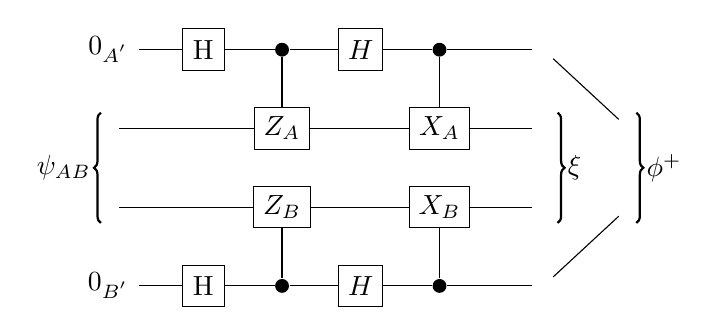
\begin{tikzpicture}
    %
    % `operator' will only be used by Hadamard (H) gates here.
    % `phase' is used for controlled phase gates (dots).
    % `surround' is used for the background box.
    \tikzstyle{operator} = [draw,fill=white,minimum size=1.5em] 
    \tikzstyle{phase} = [fill,shape=circle,minimum size=5pt,inner sep=0pt]
  % \tikzstyle{surround} = [fill=blue!10,thick,draw=black,rounded corners=2mm]
  %
  % Qubits
  \node at (0.3,0) (q1) {$\ket{0}_{A^{'}}$ };
  %\node at (0,-1) (q11) {$\ket{+}^{\rC_i''}$ };
  \node at (0.3,-1) (q2) {};
  \node at (0.3,-2) (q3) {};
  \node at (0.3,-3) (q4) { $\ket{0}_{B^{'}}$};
  \draw[decorate,decoration={brace, mirror},thick] (0.2,-0.8) to 	node[midway,left] (bracket) {$\ket{\psi}_{AB}$} (0.2,-2.2);
    % Column 1
    %\node[phase] (phase11) at (1.5,0) {} edge [-] (q1);
    %\node[operator] (phase12) at (1.5,-1) {${\tilde{\X}}_{1,A}$} edge [-] (q2);
    %\draw[-] (phase11) -- (phase12);
    %\node[phase] (phase13) at (1.5,-3) {} edge [-] (q4);
    %\node[operator] (phase14) at (1.5,-2) {${\tilde{\X}}_{1,B}$} edge [-] (q3);
    %\draw[-] (phase13) -- (phase14);
    % Column 2
    \node[operator] (op12) at (1.5,0) {H} edge [-] (q1);
    \node[operator] (op22) at (1.5,-3) {H} edge [-] (q4);
    %
 % Column 3
    \node[phase] (phase21) at (2.5,0) {} edge [-] (op12);
    \node[operator] (phase22) at (2.5,-1) {$Z_A$} edge [-] (q2);
    \draw[-] (phase21) -- (phase22);
    \node[phase] (phase23) at (2.5,-3) {} edge [-] (op22);
    \node[operator] (phase24) at (2.5,-2) {$Z_B$} edge [-] (q3);
    \draw[-] (phase23) -- (phase24);
     % Column 4
    \node[operator] (op14) at (3.5,0) {$H$} edge [-] (phase21);
    \node[operator] (op24) at (3.5,-3) {$H$} edge [-] (phase23);
    %  
 % Column 5
    \node[phase] (phase31) at (4.5,0) {} edge [-] (op14);
    \node[operator] (phase32) at (4.5,-1) {$X_A$} edge [-] (phase22);
    \draw[-] (phase31) -- (phase32);
    \node[phase] (phase33) at (4.5,-3) {} edge [-] (op24);
    \node[operator] (phase34) at (4.5,-2) {$X_B$} edge [-] (phase24);
    \draw[-] (phase33) -- (phase34);
%
    \node (end1) at (5.8,0) {} edge [-] (phase31);
    %\node (end5) at (9,-1) {} edge [-] (op81); 
    \node (end2) at (5.8,-1) {} edge [-] (phase32);
    \node (end3) at (5.8,-2) {} edge [-] (phase34);
    %\node (end6) at (9,-4) {} edge [-] (op82);
    \node (end4) at (5.8,-3) {} edge [-] (phase33);
    %
    % Bracket
    \draw[decorate,decoration={brace},thick] (6,-0.8) to 	node[midway,right] (bracket) {$\ket{\xi}$} (6,-2.2);
    \node at (5.82,0) (eend1) {};
    \node at (6.9,-1) (eend11) {};
    \draw[-] (eend1) -- (eend11);
    \node at (5.82,-3) (eend4) {};
    \node at (6.9,-2) (eend44) {};
    \draw[-] (eend4) -- (eend44);
    \draw[decorate,decoration={brace},thick] (7,-0.8) to 	node[right] (bracket) {$\ket{\phi^{+}}$} 	(7,-2.2);
    %
    % Background Box
  %  \begin{pgfonlayer}{background} 
  % \node[surround] (background) [fit = (q1) (op31) (bracket)] {};
  %  \end{pgfonlayer}
    %
\end{tikzpicture}
    \caption{Swap gate isometry used to self-test the maximally entangled state of two qubits.}
    \label{fig:swap}
\end{figure}


\subsection{CHSH correlations}


Consider outputs $a,b \in \{-1,1\}$, and inputs $x,y \in \{0,1\}$. 
Letting $\{A_x\}$ be the set of Alice's measurement observables (where $A_x = M_{1|x} - M_{-1|x}$
with $M_{a|x}$ the measurement operators), and $\{B_y\}$ the one of Bob, one can express the
expected
correlations as
\begin{equation} 
\begin{aligned} 
    \bra{\Phi} A_0\otimes B_0 \ket{\Phi} & = \dfrac{1}{\sqrt{2}} &\ 
    ,\  & \bra{\Phi} A_0\otimes B_1 \ket{\Phi} & = &\ \dfrac{1}{\sqrt{2}}  \\ 
    \bra{\Phi} A_1\otimes B_0 \ket{\Phi} & = \dfrac{1}{\sqrt{2}} &\
    ,\  & \bra{\Phi} A_1\otimes B_1 \ket{\Phi} & = & - \dfrac{1}{\sqrt{2}}  \\ 
    \bra{\Phi} A_x\otimes \mathbbm{1_B} \ket{\Phi} & = 0\   \forall x &\ ,\  
    & \bra{\Phi} \mathbbm{1_A}\otimes B_y \ket{\Phi} & = & \ 0 \  \forall y \text{.}
\end{aligned} \label{eq:corr_chsh}
\end{equation}


These correlations can be obtained if Alice and Bob share the quantum state 
\begin{equation}
    \ket{\Phi} = \dfrac{1}{\sqrt{2}} \big( \ket{00} +\ket{11}\big) \text{ ,}
\end{equation} and if Alice measures $A_0 = X$ and $A_1 = Z$, and Bob measures $B_0 = (Z+X)/\sqrt{2}$ and $B_1 = (X-Z)/\sqrt{2} $.  These operators can be related to
the measurement operators considered in \sref{Proposition}{prop:qu_corr} by
\begin{equation}
    A_x = M_{1|x} - M_{-1|x} \; \text{and} \; B_y = N_{1|y} - N_{-1|y}
\end{equation} and therefore, with \Autoref{eq:qu_corr},  we can write
\begin{equation}
    \bra{\Phi} A_{x} \otimes B_{y} \ket{\Phi} = \sum_{a,b} ab \ p(a,b|x,y)
    \label{eq:corr_to_prob}
\end{equation}
and the vector $\mathcal P = \left\{ p(a,b|x,y)\right\}$ can be derived by solving
the systems of equations defined by Equations \ref{eq:corr_chsh} and
\ref{eq:corr_to_prob}, and the normalization constraints in
Equations \ref{eq:norm_cons_1} and \ref{eq:norm_cons_2}. 

With local correlations, the following Bell inequality stands \cite{bell_einstein_1964}
\begin{equation} \label{eq:chsh}
     \left< A_0 B_0\right> + \left< A_1 B_0\right> + \left< A_0 B_1 \right> - \left< A_1 B_1 \right>  \leq 2,
\end{equation} 
which will be referred to as the CHSH inequality.

On the other hand, with a quantum behaviour the Tsirelson's inequality is always fulfilled, and  \cite{cirelson_quantum_1980}
\begin{equation}
    \left< A_0 B_0\right> + \left< A_1 B_0\right> + \left< A_0 B_1 \right>  - \left< A_1 B_1 \right>  \leq 2 \sqrt{2},
\end{equation} 
for which the upper bound, called the Tsirelson's bound, is achieved by the previous shared state and measurement.

Therefore, the quantum strategy mentioned above achieves a maximum violation of the Bell
\sref{Inequality}{eq:chsh},


\subsection{Mayers-Yao correlations}

For Mayers-Yao's self-test, the inputs are $x,y \in \{0,1,2\}$, the possible outputs
$a,b \in \{0,1\}$ and the expected correlations

\begin{equation}\label{eq:mayers-yao-correlations}
\begin{aligned}
 &\bra{\Phi} A_z \otimes B_z \ket{\Phi} & = 1 &\ \forall z \in \{0,1,2\} \\
\bra{\Phi} A_x \otimes \mathbbm{1} \ket{\Phi}  = & \bra{\Phi} \mathbbm{1} \otimes B_y \ket{\Phi} & = 0  &\ \forall x,y  \\ 
\bra{\Phi} A_0 \otimes B_1 \ket{\Phi} = & \bra{\Phi} A_1 \otimes B_0 \ket{\Phi} & = 0  &\\ 
\bra{\Phi} A_0 \otimes B_2\ket{\Phi} = & \bra{\Phi} A_1 \otimes B_2 \ket{\Phi} & = \dfrac{1}{\sqrt{2}} &\\ 
\bra{\Phi} A_2 \otimes B_0 \ket{\Phi} = & \bra{\Phi} A_2 \otimes B_1 \ket{\Phi} & = \dfrac{1}{\sqrt{2}} \text{.} & \\ 
\end{aligned}
\end{equation}


These correlations can be achieved whenever Alice and Bob share the state 
\begin{equation*}
    \ket{\Phi} = \dfrac{1}{\sqrt{2}} \left( \ket{00} +\ket{11}\right)\text{,}
\end{equation*}
and their measurement observables are 
\begin{equation*}
\begin{aligned}
        A_0 = X_A   \ , \  A_1 = Z_A  , \ A_2 = \dfrac{1}{\sqrt{2}}  (X_A + Z_A), \\
        B_0 = X_B   , \  B_1 = Z_B  \ , \ B_2 = \dfrac{1}{\sqrt{2}}  (X_B + Z_B) .\\
\end{aligned}
\end{equation*}

\newpage